\chapter{General Concepts}
\section{Classification of Second order PDEs} % (fold)
\subsection{General Problem} % (fold)
\label{sub:General Problem}
For PDEs of order above one no general methods exist to solve them
and methods for solving differ quite a bit from each other,
thus PDEs are classified by methods that solve them and once
a new method to solve is found all pdes that can be solved
by it are classified under it.\\[1ex]

A general second order linear PDE has the following form :
\begin{definition}[Second Order Linear PDE]
	A general second order linear PDE is given by :
	\begin{align*}
		Lu(x) = \sum_{i,j=1}^{n}  a_{i,j}(x) \partial_i \partial_j u +  \sum_{i=1}^{n}  b_{i}(x) \partial_i u + c(x)u(x) = 0
		.\end{align*}
	i.e, second order terms , first order terms and 0th order terms. \\[1ex]
	Where $a_{i,j}$ is a matrix of coefficients and pde's can be classified by the shape they take.
	The matrix $a_{i,j}$ is symmetric and diagonalizable as the partial derivatives are symetric \textbf{Schwarz's Theorem} ($a_{i,j} \equiv \frac{1}{2}(a_{i,j} + a_{j,i})$)
\end{definition}
% subsection General Problem (end)
\label{sec:Classification of Second order PDEs}
\subsection*{Elliptic PDEs} % (fold)
\label{sub:Elliptic PDEs}
\begin{definition}[Elliptic PDEs]
	If the matrix $a_{i,j}$  is the unity matrix and $b=c=0$ then they are called elliptic pdes
\end{definition}
\begin{example}[Laplace Equation]
	Laplace Equation is given by :
	\begin{align*}
		\triangle u \coloneqq \frac{\partial^2 u}{\partial x_1^2} +\ldots + \frac{\partial^2 u}{\partial x_n^2} = 0
		.\end{align*}
	Solutions are called harmonic functions. Important tool : a priori estimates i.e lower order derivatives can be estimated in terms of second order derivatives.
\end{example}
Major example whose investigation played a role in the development of elliptic theory is :
\begin{example}[Minimal surface equation]
	Note $\triangledown * u  $ =  $\begin{pmatrix} \frac{\partial }{\partial x_1},\ldots, \frac{\partial }{\partial x_n}   \end{pmatrix} * \begin{pmatrix} u_1 \\ \vdots \\ u_n \end{pmatrix} $ \\[1ex]
	\begin{align*}
		\triangledown * \frac{\triangledown u }{\sqrt{1 + \abs{\triangledown u  }^2} }
		.\end{align*}
	The graphs of such solutions describe minimal surfaces. The area of such hypersurfaces in $\mathbb{R}^{n+1} $ does not change with infinitesimal variation. \\[1ex]
	\textbf{Example : } Soap bubbles are one example. \\[1ex]
	Boundary value problem is called Plateaus problem, first proof of existence received Field's Medal (Jesse Douglas)
\end{example}
% subsection Elliptic PDEs (end)
\subsection{Parabolic PDEs} % (fold)
\label{sub:Parabolic PDEs}
Parabolic PDEs are linear PDEs where the matrix $a_{i,j}$ is considered as a symmetric
bilinear form which is only semi-definite and belong to the boundary of the class of elliptic PDEs.
semi-definite (all eigenvalues are non-negative / non positive).
\begin{example}[Heat equation]
	The heat equation is given by :
	\begin{align*}
		\dot{u} - \triangle u = 0
		.\end{align*}
	And describes diffusion processes, named after the prominent example of temperature.\\
	Many stochastic processes have this property. \\[1ex]
	These are processes which level inhomogeneities of some quantity by some flow along the negative gradient of the quantity.\\
	\textbf{Interpretation : }  the rate $\dot{u}$ at which the material at a point will heat up (or cool down) is proportional
	to how much hotter (or cooler) the surrounding is.\\
\end{example}
\begin{comment}
Tools of Laplace equation can be applied in modified form to this heat equation
\end{comment}
\begin{example}[Ricci Flow]
	\begin{align*}
		\dot{g}_{i,j} = -2R_{i,j}
		.\end{align*}
	This PDE describes a diffusion-like process on Riemannian manifolds, it levels the inhomogeneities of the metric (g).
\end{example}
\begin{definition}{Riemannian Manifold}
	A Manifold is a  locally euclidean space but not globally, common example are maps of an atlas,
	i.e we can locally embed the maps into $\mathbb{R}^{n} $ but globally thats impossible, a Riemanniann manifold is
	a $n$ dimensional manifold with a function $g$ that assigns every point $p \in  M$  a scalar product.
\end{definition}
% subsection Parabolic PDEs (end)
\subsection{Hyperbolic PDE} % (fold)
\label{sub:Hyperbolic PDE}
Hyperbolic PDEs are the second most important class of linear PDEs.
The matrix $a_{i,j}$ has one eigenvalue of opposite sign than all other eigenvalues.
An example is :
\begin{example}[Wave equation]
	\begin{align*}
		\frac{\partial^2 u}{\partial t^2} - \triangle u = 0
		.\end{align*}
	The wave equation describes the behavior of waves with constant finite speed.
	The investigation of these PDEs depend on understanding all trajectories which propagate by given speed.
\end{example}

% subsection Hyperbolic PDE (end)
% section Classification of Second order PDEs (end)
\section{Existence of Solutions} % (fold)
\label{sec:Existence of Solutions}
There exists PDEs with smooth coefficients without solutions, an example to this is :
\begin{align*}
	\frac{\partial u}{\partial x}  + i \frac{\partial u}{\partial y} = f(x,y)
	.\end{align*}
Sucht that :
\begin{align*}
	 & f(-x,y) = f(x,y)                                                                                                                                                             \\
	 & \text{there exists a sequence of positive numbers $\rho_n \downarrow 0 $,such that f vanishes on a neighbourhood of the circles boundary $\partial B(0,\rho_n)$  in contrast
		to non vaninishing integrals $\int_{B(0,\rho_n)} f(x,y) dx dy \neq  0$  }
	.\end{align*}
The idea to proof there exists no solution in a neighbourhood of $(0,0) \in  \mathbb{R}^2$ is to :
\begin{enumerate}
	\item If the function $u(x,y)$ is a solution then due to (i) $-u(-x,y)$ is also a solution.
	      Such that $u \equiv frac{1}{2}(u(x,y)-u(-x,y))$ and assume $u(-x,y) = -u(x,y)$
	\item We claim that every solution u vanishes on the circles boundary $\partial B(0,\rho_n)$.
\end{enumerate}
This leads to a contradiction by the Divergence Theorem :
\begin{align*}
	\int_{B(0,\rho_n)} f dx dy & = \int_{B(0,\rho_n)} (\frac{\partial u}{\partial x} +i x \frac{\partial u}{\partial y}  ) dx dy = \int_{B(0,\rho_n) \triangledown * \begin{pmatrix} u \\ ixu \end{pmatrix} } dx dy \\
	                           & \myS{Div Th.}{=} \int_{\partial B(0,\rho_n)} \begin{pmatrix} u \\ ixu \end{pmatrix} * N(x,y) d\sigma(x,y) = 0                                                                      \\
	.\end{align*}
% section Existence of Solutions (end)
\section{Regularity of Solutions} % (fold)
\label{sec:Regularity of Solutions}
Regularity of a differential equation refers to the local properties of the corresponding functions.
The most general functions we consider are distributions, which have the lowest regularity.\\[1ex]
Distributions contain measurable functions with the next highest regularity.
The highest regularity are smooth functions and analytic functions.
% section Regularity of Solutions (end)
\section{Boundary Value Problems} % (fold)
\label{sec:Boundary Value Problems}
In general partial differential equations have an infinite dimensional space of solutions.
Similar to how solutions in the ODE case can be uniquely determined (by fixing the values of the derivatives),
in PDEs solutions are functions on higher dimensional domains $\Omega  \subset  \mathbb{R}^{n}  $ such that a natural condition is the specification of the values of the solution
and some of its derivatives on the boundary of the domain.
% section Boundary Value Problems (end)
\section{Divergence Theorem} % (fold)
\label{sec:Divergence Theorem}
The divergence theorem is a generalization of the fundamental theorem of calculus to higher dimensions.
It states that the surface integral of a vector field over a closed surface, 
which is called the "flux" through the surface, is equal to the volume integral of the divergence over the region inside the surface.
The Idea behind it can be classified into two definitions 
\begin{definition}
 A continuously differentiable homeomorphism $\Phi : \mathbb{R}^{k } \supset U \to A \subset  \mathbb{R}^{n }  $ 
 is called a $k-$dimensional parameterization of A. It is called regular if the Jacobian $\phi'$ has full rank k at every point of U.
\end{definition}
\begin{comment}
 The Idea is that, given a Shape A we find a function $\Phi $ that parameterizes this shape such that we can integrate it. 
\end{comment}
\begin{definition}
 Let $A \subset  \mathbb{R}^{n } $ be a subset with a regular parameterization $\Phi $ and f a continuous function on A. 
 We define : 
 \begin{align*}
   \int_A f d\sigma  \coloneqq  \int_U f \circ \Phi \sqrt{det((\Phi')^{T}\Phi') } d\mu_{\mathbb{R}^{k} }
 .\end{align*}
 $\Phi'$ is the Jacobian.
\end{definition}
\begin{comment}
The $\sqrt{det} $ factor measures the distortion of the parameterization and is independent of the choice of regular parameterisation of A.
This definition gives us a concrete integral to compute, as long as it can be regularly parameterised
\end{comment}
Some subsets cannot be regularly parameterised, usually this is because the cannot be covered by a single parameterisation an example of this 
is a sphere, as a sphere is compact there cannot exists a homeomorphism between the sphere and any open set $U \subset  \mathbb{R}^{k } $
this can be solved by using more than one parameterisation, thus the following definition
\begin{definition}[Submanifold]
  A subster $A \subset  \mathbb{R}^{n } $ is called a $k-$dimensional submanifold if there exists 
  subsets $A_i$ such that each $A_i$ has a regular $k-$dimensional parameterization and $A = \cup A_i$
\end{definition}
Issue : subsets can overlap ,which leads to double counts when integrating over the parameterisations.
An answer to this are partitions of unity (not practically useful)
\begin{definition}
  Let $\Omega  \subset  \mathbb{R}^{n } $ be covered by a countable family $U_{i \in  \mathbb{N}}$ of open subsets.
  A smooth partition of unity is a countable family $(h_i)_{i \in  \mathbb{N}}$ of smooth functions $h_i : \Omega  \to [0,1]$ such that : 
  \begin{enumerate}
    \item Each $x \in  \Omega $ has a neighbourhood on which all but finite many $h_i$ vanish identically
    \item For all $x \in  \Omega $ we have $\sum_{i=1}^{\infty} h_i(x) = 1$
    \item Each $h_i$ vanishes outside of $U_i$
  \end{enumerate}
  For every family of open subsets of $\mathbb{R}^{n} $ there exists a smooth partition of unity.
\end{definition}
\begin{theorem}[Divergence Theorem ]
  Let $\Omega \subset  \mathbb{R}^{n }  $ be bounded and open with $\partial \Omega $ being a 
  $(n-1)-$ dimensional sub-manifold of $\mathbb{R}^{n } $. Let $F : \overline{\Omega}  \to  \mathbb{R}^{n } $ be continuous and 
  differentiable on $\Omega $ such that $\triangledown F$ continuously to $\partial \Omega $. Then we have : 
  \begin{align*}
    \int_{\Omega } \triangledown * F d\mu = \int_{\partial \Omega } F * N d\sigma
  .\end{align*}
  where N is the outward pointing normal. (last component is positive)
\end{theorem}
\begin{proof}
 First Note that $\triangledown * F = \partial_1 F_1 + \ldots  + \partial_n F_n$ 
 Idea is to do the proof component wise and proof a statement about each component and put them back together\\[1ex]
 In the special case of $F,F' =0$ on the boundary then extend F by 0 to $\mathbb{R}^{n} $ to show that the both sides vanish. We know $\Omega $ is bounded and as such is contained by a Box and by continous extension we can integrate over that box 
 \begin{align*}
   \int_\Omega  \triangledown * F = \int_{\text{Box}} \triangledown * F =  \sum \int_{\text{box}} \partial_i F_i 
 .\end{align*}
 Where 
 \begin{align*}
   \int_{\text{box}} \partial_i F_i &= \int_{-R}^{R}\iint_{-R}^{R}   \partial_i F_i dx_1 dx_2 \ldots  dx_n \\
                                    &= \iint [\int_{-R}^{R} \partial_i F_i ]_{-R}^{R}   = 0\\ 
 .\end{align*}
 Such that the sum is 0 as well \\[1ex]
 In the general case we do it similar , where the existence of the box is guaranteed by the fact that every submanifold is a graph over some box.
 We are able to cover $\overline{\Omega } $ by $\Omega $ and all the boxes $V' \times  (a,b) \subset  \mathbb{R}^{n}  $, by compactness we only need finite many 
 sets to cover $\overline{\Omega } $, by choosing a partition of unity we avoid including the same point multiple times : 
 \begin{align*}
   \int_{\partial \Omega } F*N d \sigma  = \sum \int_{\partial \Omega \cap U_i } (h_i * F) N d \sigma  
 .\end{align*}
 Remember that each $h_i$ vanishes outside $U_i$, in the case $U_i = \Omega $ then $h_i F$ is 0 on the boundary and is covered by the first case.
 Normal case is $U_i = V' \times  (a,b)$ for some $a,b$
 \begin{figure}[H]
 \begin{center}
 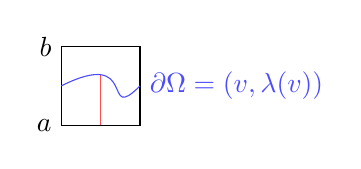
\begin{tikzpicture}
   \draw[] (0,0) -- (1,0) -- (1,1) -- (0,1) -- (0,0);
   \node[left] (a) at (0,0) {$a$};
   \node[left] (b) at (0,1) {$b$};
   \draw[red!70] (1/2,0) -- (1/2,2.55/4);
   \draw[blue!70] (0,1/2) .. controls (1,1) and (0.5,0) .. (1,1/2) node[right,blue!70] {$\partial \Omega  = (v,\lambda(v))$};
 \end{tikzpicture} 
 \end{center} 
 \end{figure}
 Where the area below the curve is $\Omega $ in essence we integrate over lines : 
 \begin{align*}
  x \mapsto \int_a^{\lambda(x)}  F_i(x,z) dz
 .\end{align*}
 Note that $\lambda(x)$ is the height at point x such that the integral of the $\partial_i$ term :
 \begin{align*}
   \int_{\Omega  \cap U_i} \partial_i F_i = \int_{V'} \int_a^{\lambda(x)}  \partial_{x_i} F_i(x,z) dz d^{n-1} x  = \int_{V'} \lambda(x)*F_i(x,\lambda(x)) d^{n-1}x
 .\end{align*}
 Last equality follows from the fact that F is zero on $V' \times  \{a\}  $ (by property of the partition of unity $h_i$ 
\end{proof}
\begin{definition}[Formula outward pointing Normal]
  The formula for the outward pointing normal is given by 
  \begin{align*}
    N =  \pm \frac{1}{\sqrt{1+\abs{\triangledown \lambda}}^2 }\begin{pmatrix} -\triangledown \lambda  \\ 1 \end{pmatrix} 
  .\end{align*}
  Where $\lambda $ is a height function,this says in essence that every sub manifold is a graph over a coordinate plane. The explicit formula of $N$ comes from the fact 
  that we can determine every tangent and then just determine N such that the dualproduct (dot product) is 0 
\end{definition}
\begin{comment}
 The symbol $d\sigma$ in this case means that the integral is a surface integral and not a classical integral on a subset of $\mathbb{R}^{n } $.
\end{comment}
\begin{definition}[Projection ]
  Let $P$ be a projection otno the jth coordinate
  \begin{align*}
    P(x) = (x_{1},\ldots ,\underbrace{c}_{jth},\ldots x_n)
  .\end{align*}
  To get the derivative is just the identity except at the jth coordinate where it is 0  \\[1ex] 
  Now if there exists a regular parameterization of the plane $\Phi  : \mathbb{R}^{k} \to \mathbb{R}^{n}   $  to get a regular parameterization
  we can project onto the coordinate which would not be linear independent which gives us full rank
\end{definition}
\begin{example}
 How does the divergence theorem genrealize the fundamental theorem of calculus , 
 we consider a scalar valued function $f$ and embed it into a vector valued funciton $F = \begin{pmatrix} 0 , \ldots  , f , \ldots  0 \end{pmatrix} $ 
 then 
 \begin{align*}
   \int_{\Omega } \partial_i f d\mu  = \int_{(a,b)} \partial_i f  d\mu  = \int_{\{a,b\}  }f N_i d\sigma  = (fN_i)(a) + (fN_i)(b) = f(b)-f(a)
 .\end{align*}
\end{example}
\begin{example}[Volume of unit ball]
  Volume of unit ball in $n$ dimension is given by the volume of the unit ball scaled by $r^{n} $ and some cosntant $\omega_n$, 
\end{example}

% section Divergence Theorem (end)
\section{Distributions} % (fold)
\label{sec:Distributions}
Main trick is to use integration by parts to "transfer" the integration from one function to the other, see : 
\begin{align*}
  F_f(\Phi) =  \int_\Omega f \Phi d\mu 
.\end{align*} 
\begin{align*}
  F_{f'}(\Phi) = \int_\Omega f' \Phi  d\mu  = -\int_\Omega f \Phi' d\mu  
.\end{align*}
Where the boundary terms vanish as $\Phi $ is a test function, that vanish on outside of a compact set ?.\\[1ex]
In general distributions are a way to define solutions for partial differential equations 
that may not posses a regular solution that is continuously differentiable. Thus distributions are a special case of functions 
that act as weak solutions for linear differential equations  (solutions in the sense of distributions )
\subsection{Test Functions} % (fold)
\label{sub:Test Functions}
Test functions are infinitely differentiable functions that vanish outside of their compact support.
We say for an open set $\Omega  \subset \mathbb{R}^{n } $ the set of test functions $\mathcal{D}(\Omega )$ are such functions with the following 
notion of convergence : 
We say test functions converge $f_n \to f $ if there is a compact subset $K \subset  \Omega $ such that $\forall n \in  \mathbb{N} \ : \ supp f_n \in K$ and 
$\partial t ^{\alpha }f_n \to \partial ^{\alpha } f $ in the supremum norm on K for every multi-index $\alpha $.
\subsubsection{Mollifier}
Mollifier or approximate identities is a subset of test functions $(\lambda_{\epsilon })_{\epsilon  > 0}$ with 
$supp \lambda_\epsilon  = \overline{B(0,\epsilon )}$ and $\int  \lambda_\epsilon  d\mu  = 1$, the standard molifier is defined as : 
\begin{align*}
  \lambda(x) \coloneqq  \begin{cases}
    C\exp(\frac{1}{\abs{x}^2-1}), &\text{ if }\abs{x} < 1 \\
    0 &\text{ if } \abs{x}>1
  \end{cases}
.\end{align*}
Then the standard mollifier is given by : 
\begin{align*}
  \lambda_\epsilon(x) = \epsilon ^{-n} \lambda (\frac{x}{\epsilon }) 
.\end{align*}
They have the property that for any continuous function $f$ on $\Omega $ and suppose $0 \in \Omega $ then : 
\begin{align*}
  \int_\Omega  f \lambda_\epsilon  d\mu  \approx \int_{B(0,\epsilon )} f(0)\lambda_\epsilon d\mu  = f(0)
.\end{align*}
This is in fact an equality as $\epsilon  \downarrow 0 $, the proof can be summarized as 
choosing a compact subset of $\Omega $ then taking an $\epsilon $ ball around any point x such that the Ball $B(x,\epsilon ) \subset \Omega $: 
\begin{align*}
  \abs{f_{\epsilon }(x) - f(x)} = \abs{\int_\Omega  \lambda_\epsilon (x-y)(f(y)-f(x)) d^{n} y } \le \sup_{y \in  B(x,\epsilon )} \abs{f(y)-f(x)}   
.\end{align*}
when $\epsilon  \downarrow 0 $ the sup goes to 0 uniformly.\\[1ex]
\textbf{Usecase : } Mollifiers are used to prove  that properties valid for smooth functions are also valid in nonsmooth situations
and in our case to give notion to product of distributions.
% subsection Test Functions (end)
\subsection{Formal Definition } % (fold)
\label{sub:Formal Definition }
\begin{definition}
  For any function $f \in  L_{loc}^{1}(\Omega ) $  a distribution is given by : 
  \begin{align*}
    F_f : \mathcal{D}(\Omega ) \to  \mathbb{R}, \qquad \Phi \mapsto \int_\Omega  f \Phi  d \mu 
  .\end{align*}
\end{definition}
We define the space of distributions as  
\begin{definition}
  On an open subset $\Omega  \subset  \mathbb{R}^{n} $  the space of distributions $\mathcal{D}'(\Omega )$ is 
  defined as the vector space of all linear maps $F: \mathcal{D}(\Omega ) \to \mathbb{R}$ which are continuous with respect to the 
  seminorms 
  \begin{align*}
    \|\cdot \|_{K,\alpha } : \mathcal{C}_0^{\infty}(\Omega ) \to \mathbb{R} \qquad \Phi  \mapsto \|\Phi \|_{K,\alpha } \coloneqq \sup_{x \in  K} \abs{\partial ^{\alpha } \Phi(x) }
  .\end{align*}
  meaning for each compact $K \subset  \Omega $ there exist finite many multiindicies $\alpha_i$ and constants $C_i >0$ such that the following holds 
  for all testfunctions $\Phi  \in  \mathcal{D}(\Omega )$ : 
  \begin{align*}
    \abs{F(\Phi )} \le  C_1\|\Phi \|_{K,\alpha_1} + \ldots + C_M\|\Phi \|_{K,\alpha_M}
  .\end{align*}
  The space of distributions $\mathcal{D}'$ can be regarded as the dual space of $\mathcal{D}$
\end{definition}
\begin{corollary}
 We get the following convergence property : \\[1ex]
 If $\Phi_n \to  \Phi $ in $\mathcal{D}(\Omega )$ then the values  $F(\Phi_n) \to  F(\Phi )$ and 
 we say a sequence of distributions $F_n$ converges to F if $F_n(\Phi ) \to F(\Phi )$ for all test functions $\Phi $
\end{corollary}
\begin{definition}
 The delta distortion is a special case of distortion such that it does not correspond to an element of $L_{loc}^{1 }(\mathbb{R}^{n } ) $ : 
 \begin{align*}
   \delta  : \mathcal{D}(\mathbb{R}^{n} ) \to \mathbb{R} \qquad \Phi  \mapsto \Phi(0)
 .\end{align*}
 It is the limit of the sequence of distributions corresponding to the mollifier $\lambda_\epsilon $
\end{definition}
% subsection Formal Definition  (end)
\subsection{Opereations on Distributions} % (fold)
\label{sub:Opereations on Distributions}
The goal is to define as many operations on  distributions as possible.
The first operation we define is convolution, by first defining it on $\mathcal{C}_0^\infty(\mathbb{R}^{n} )$
\begin{align*}
  (g \star f)(x) \coloneqq  \int_{\mathbb{R}^{n } }  g(x-y)f(y) d^{n }y = \int_{\mathbb{R}^{n } }g(z)f(x-z) d^{n} z
.\end{align*}
by using integration by parts we get : 
\begin{align*}
  \partial ^{\alpha }(g \star f) = (\partial ^{\alpha } g ) \star  f = g \star (\partial ^{ \alpha }f ) 
.\end{align*}
convolution is well behaved in respect to integration by using volume preserving transformation $z=y-x , y=y$,
and preservers symmetry of functions, also proven by coordinate transformation $y=Oz+b$
% subsection Opereations on Distributions (end)


% section Distributions (end)
